\chapter{PENDAHULUAN}
\label{chap:pendahuluan}

% Ubah bagian-bagian berikut dengan isi dari pendahuluan

\section{Latar Belakang}
\label{sec:latarbelakang}

Game strategi merupakan permainan di mana pemain mengambil keputusan strategis di dalam game untuk menyelesaikan tujuan. 
Salah satu game tersebut merupakan seri \emph{Civilization}. 
\emph{Civilization VI} (Civ6) merupakan instalasi terbaru dari seri game ini. 
Civ6 adalah game strategi berbasis giliran (\emph{Turn-based strategy game}) terpopuler. 
Dalam game ini, pemain melakukan aksi bergilir dengan lawannya dalam area map yang tersusun dari lantai segi enam (\emph{hexagonal grid}).
Pemain dapat mempunyai lawan berupa manusia lain maupun sebuah agen berbasis \emph{artificial intelligence} (AI).

Civ6 merupakan game 4X (\emph{Explore, Expand, Exploit, Exterminate}). 
Dalam game ini, pemain dapat memilih negara-negara yang telah muncul dalam sejarah. 
Pemain memiliki tujuan untuk menjelajah area di dalam game yang telah dibuat secara acak (\emph{Explore}), memperluas teritori milik pemain (\emph{Expand}), memanfaatkan teritori yang dimiliki (\emph{Exploit}), dan menghancurkan teritori milik lawan (\emph{Exterminate}). 
Aspek-aspek 4X tersebut menyebabkan game ini menjadi sangat kompleks. 
Lingkungan kompleks dalam \emph{Civilization} memberikan banyak kemungkinan dalam \emph{action space} dan \emph{state space} yang luas \citep{civ4City}.
Hal ini menjadi tantangan bagi \emph{game developer} untuk membuat lawan AI yang dapat memberikan tantangan yang cukup terhadap pemain dalam lingkungan game yang kompleks seperti ini. 
Akan tetapi, game strategi 4X seperti Civ6 masih memiliki kapabilitas agen berbasis AI yang belum optimal.

\begin{figure}[H]
    \centering
      % Nama dari file gambar yang diinputkan
      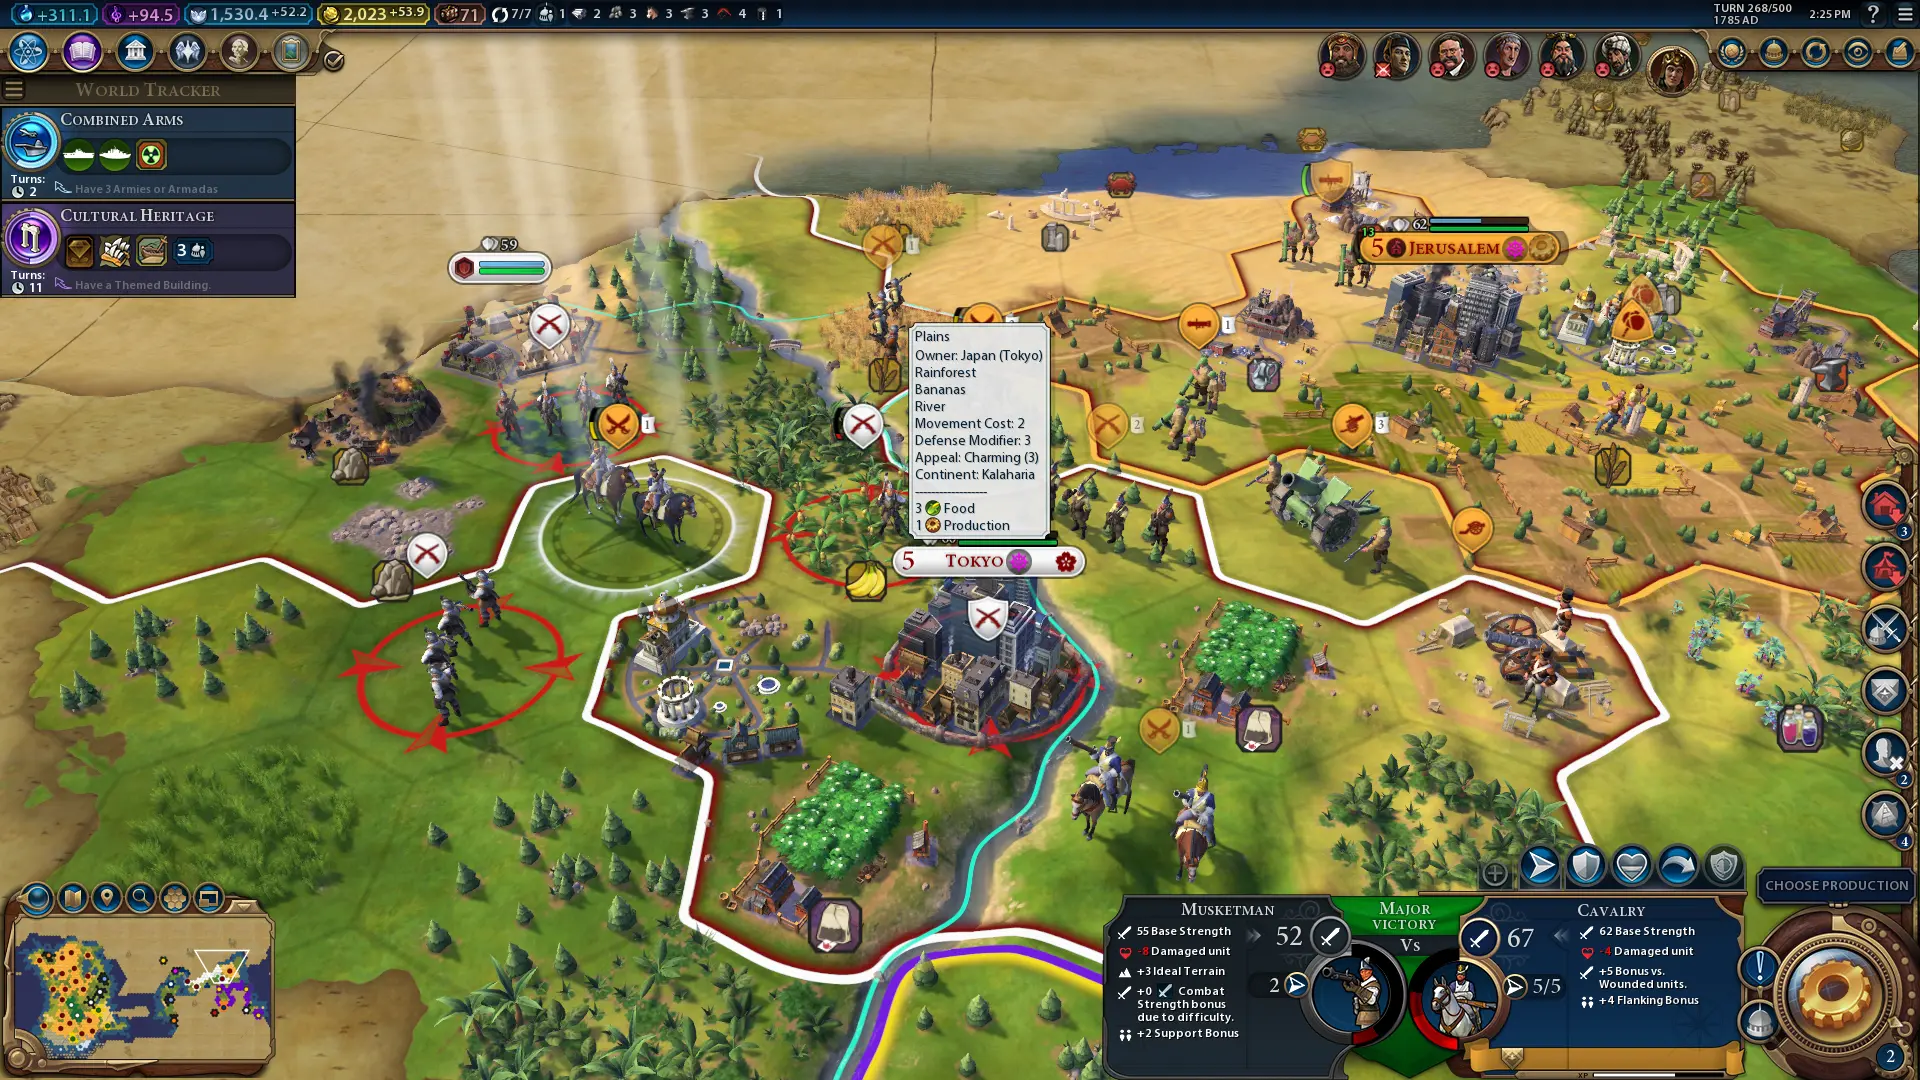
\includegraphics[scale=0.23]{gambar/civ6_screenshot.png}
      % Keterangan gambar yang diinputkan
      \caption{\emph{Combat} dalam \emph{Civilization} VI}
      % Label referensi dari gambar yang diinputkan
      \label{fig:civ6_combat_image}
  \end{figure}

Dengan mengintegrasikan teknik-teknik \emph{machine learning}, AI memiliki potensial untuk bertindak seperti kemampuan manusia \citep{humanLevelAI}.
Berkembangnya bidang \emph{Deep Reinforcement Learning} menawarkan teknologi AI yang belum memungkinkan sebelumnya. 
DRL telah digunakan untuk membuat agen AI yang mampu bermain dalam game yang kompleks dan sulit seperti Atari 2600, Dota 2, dan Starcraft 2 \citep{DRLSurvey}.

\section{Permasalahan}
\label{sec:permasalahan}

Lawan berupa agen berbasis AI dalam Civ6 saat ini mempunyai keterbatasan. 
Agen berbasis AI tersebut terpaku hanya pada aturan yang sudah diprogram, 
sehingga tidak dapat beradaptasi terhadap pemain. 
Seiring berkembangnya kemampuan pemain dalam game tersebut, 
pemain akan mendapatkan bahwa agen berbasis AI yang dilawannya sudah tidak lagi 
memberikan tantangan yang cukup. Hal ini menyebabkan sebuah fenomena bernama \emph{Chick Parabola}. 
\emph{Chick Parabola} merupakan fenomena dimana ketertarikan pemain terhadap game tersebut menurun seiring berkembangnya kemampuan pemain \citep{chickParabola}.

Kurangnya kapabilitas agen berbasis AI dalam Civ6 sangat terlihat dalam aspek \emph{combat}. 
Dalam \emph{combat}, agen berbasis AI tidak dapat memutuskan aksi unit secara optimal. 
Agen AI didapatkan sering menempatkan unit di posisi yang tidak logis. 
Aksi yang dilakukan oleh agen berbasis AI serasa acak. 
Developer Civ6 (\emph{Firaxis}) mencoba mengatasi hal ini dengan menambahkan modifiers. 
Pada tingkat kesulitan yang tinggi, agen berbasis AI akan mendapatkan modifiers berupa combat value. 
Secara praktis, bonus ini diberikan untuk menanggulangi kurangnya kemampuan taktis dan strategis agen berbasis AI. 
Solusi ini tidaklah ideal dalam game strategi yang secara desain mengedepankan kemampuan untuk berfikir dan merencanakan aksi untuk mencapai tujuan.
Diperlukanlah sebuah teknik maupun teknologi AI baru untuk mengatasi masalah ini.

\section{Batasan Masalah}
\label{sec:batasanmasalah}

Penelitian ini mencakup pada implementasi beberapa algoritma \emph{state of the art} \emph{deep reinforcement learning} dalam sebuah \emph{environment}. 
Mekanisme \emph{environment} mengikuti mekanisme \emph{combat} dalam game \emph{Civilization} 6 yang merupakan \emph{hexagonal grid turn-based strategy game} terpopuler saat penelitian ini ditulis. 
Luas \emph{environment} sebesar 8 x 8. Di tengah \emph{environment} terdapat sebuah kota yang dapat direbut oleh agen AI. 
Terdapat dua agen dalam penelitian ini, yaitu agen \emph{attacker} dan agen \emph{defender}. 
Jenis unit yang digunakan oleh agen AI berupa unit jarak dekat (\emph{warrior}) dan unit jarak jauh (\emph{slinger}). 
Kedua unit tersebut merupakan unit paling awal yang digunakan dalam \emph{Civilization} 6.
Sebuah game penuh berbasis DRL berada di luar batasan penelitian ini. 
Namun, \emph{environment} yang digunakan sebagai prototipe akan menjadi \emph{proof of concept} akan kapabilitas DRL dalam \emph{hexagonal grid turn-based strategy game}.

\section{Tujuan}
\label{sec:Tujuan}

Tujuan penelitian ini adalah mengimplementasikan dan mengukur kemampuan dari beberapa 
algoritma \emph{state of the art} \emph{deep reinforcement learning} dalam sebuah \emph{environment} yang memiliki skenario combat dan mekanisme
sebuah \emph{hexagonal grid turn-based strategy game}.

\section{Manfaat}
\label{sec:manfaat}

Hasil dari penelitian ini diharapkan dapat memberikan contoh implementasi dalam merancang 
sebuah agen AI menggunakan metode \emph{deep reinforcement learning} serta memberikan acuan performa beberapa algoritma \emph{state of the art deep reinforcement learning} kepada game developer atau game AI programmer untuk 
mengimplementasikan agen berbasis \emph{deep reinforcement learning} dalam sebuah hexagonal grid turn-based strategy game.
